\section{A Data-Capturing Metamodel}
\label{sec:dataset:architecture}

Why should we care about the architecture of our dataset capturing, so long as the \gls{ai} is well-trained? This question fundamentally leads to the \textit{provenance} or \textit{lineage} of our data: not all training data is initially perfect. At times, we will need to modify our training data, or in the cases of some \gls{ai} systems, training data is re-fed back into the system from the \gls{ai} itself. 

Hence, it is imperative to understand how the transition and flow of data occurs \citep{Cui:2003im,Ikeda:2009ca,Buneman:2000bn} in these \gls{ai} systems. Where does it comes from? How is it derived and updated, and how might this affect our trained \gls{ai} models over time? Without a thorough understanding of data provenance, tracing potential defects within training models becomes difficult. It may be a difference in the data training format, or a mismatch of values on the same training data. Systematic record-keeping is critical to overcome this challenge.

We propose a grammar to capture the vocabulary of our metamodel and the approach of developing a data-capturing architecture. As such a grammar is textual, it can be version controlled: therefore data provenance is recorded, which allows us to source how the mutations in training data can occur and and what effect this has our \gls{ai} systems. From an exploratory analysis of developing a concrete implementation of this system (\cref{sec:dataset:architecture:methodology}), we propose a conceptual metamodel that can be used to annotate and formally describe image data for training purposes (e.g., frames of a video, images of natural scenes). This metamodel is inspired by the works of \citet{Wickham:2010hy, Wickham:2007tu} and \citet{Moody:2009vo}.

\subsection{Methodology}
\label{sec:dataset:architecture:methodology}

To understand the methodology on how we captured our dataset, we must first introduce the three key notions behind \gls{mde}: technical spaces, models and systems. A system is a concrete ``group or set of related or associated elements perceived or thought of as a unity or complex whole'' \citep{oed:system}. Technical spaces were introduced \citet{Bezivin:2002} as a model management framework based on algebraic structures (e.g., trees, (hyper)graphs, categories). Technical spaces are usually based on a three-tier conjecture: metametamodels, metamodels and models. Whereas a model is an abstract representation a concrete system of specific purpose, a \textit{meta}model, in contrast, describes the way to describe those models. A \textit{metameta}model can be used to describe the representation structure of our metamodels and defines a type system that supports all underlying layers \citep{Bezivin:2006gw}. \cref{fig:dataset:bezivin2006_metamodel} captures these concepts in further detail.

\begin{figure}[h]
  \centering
  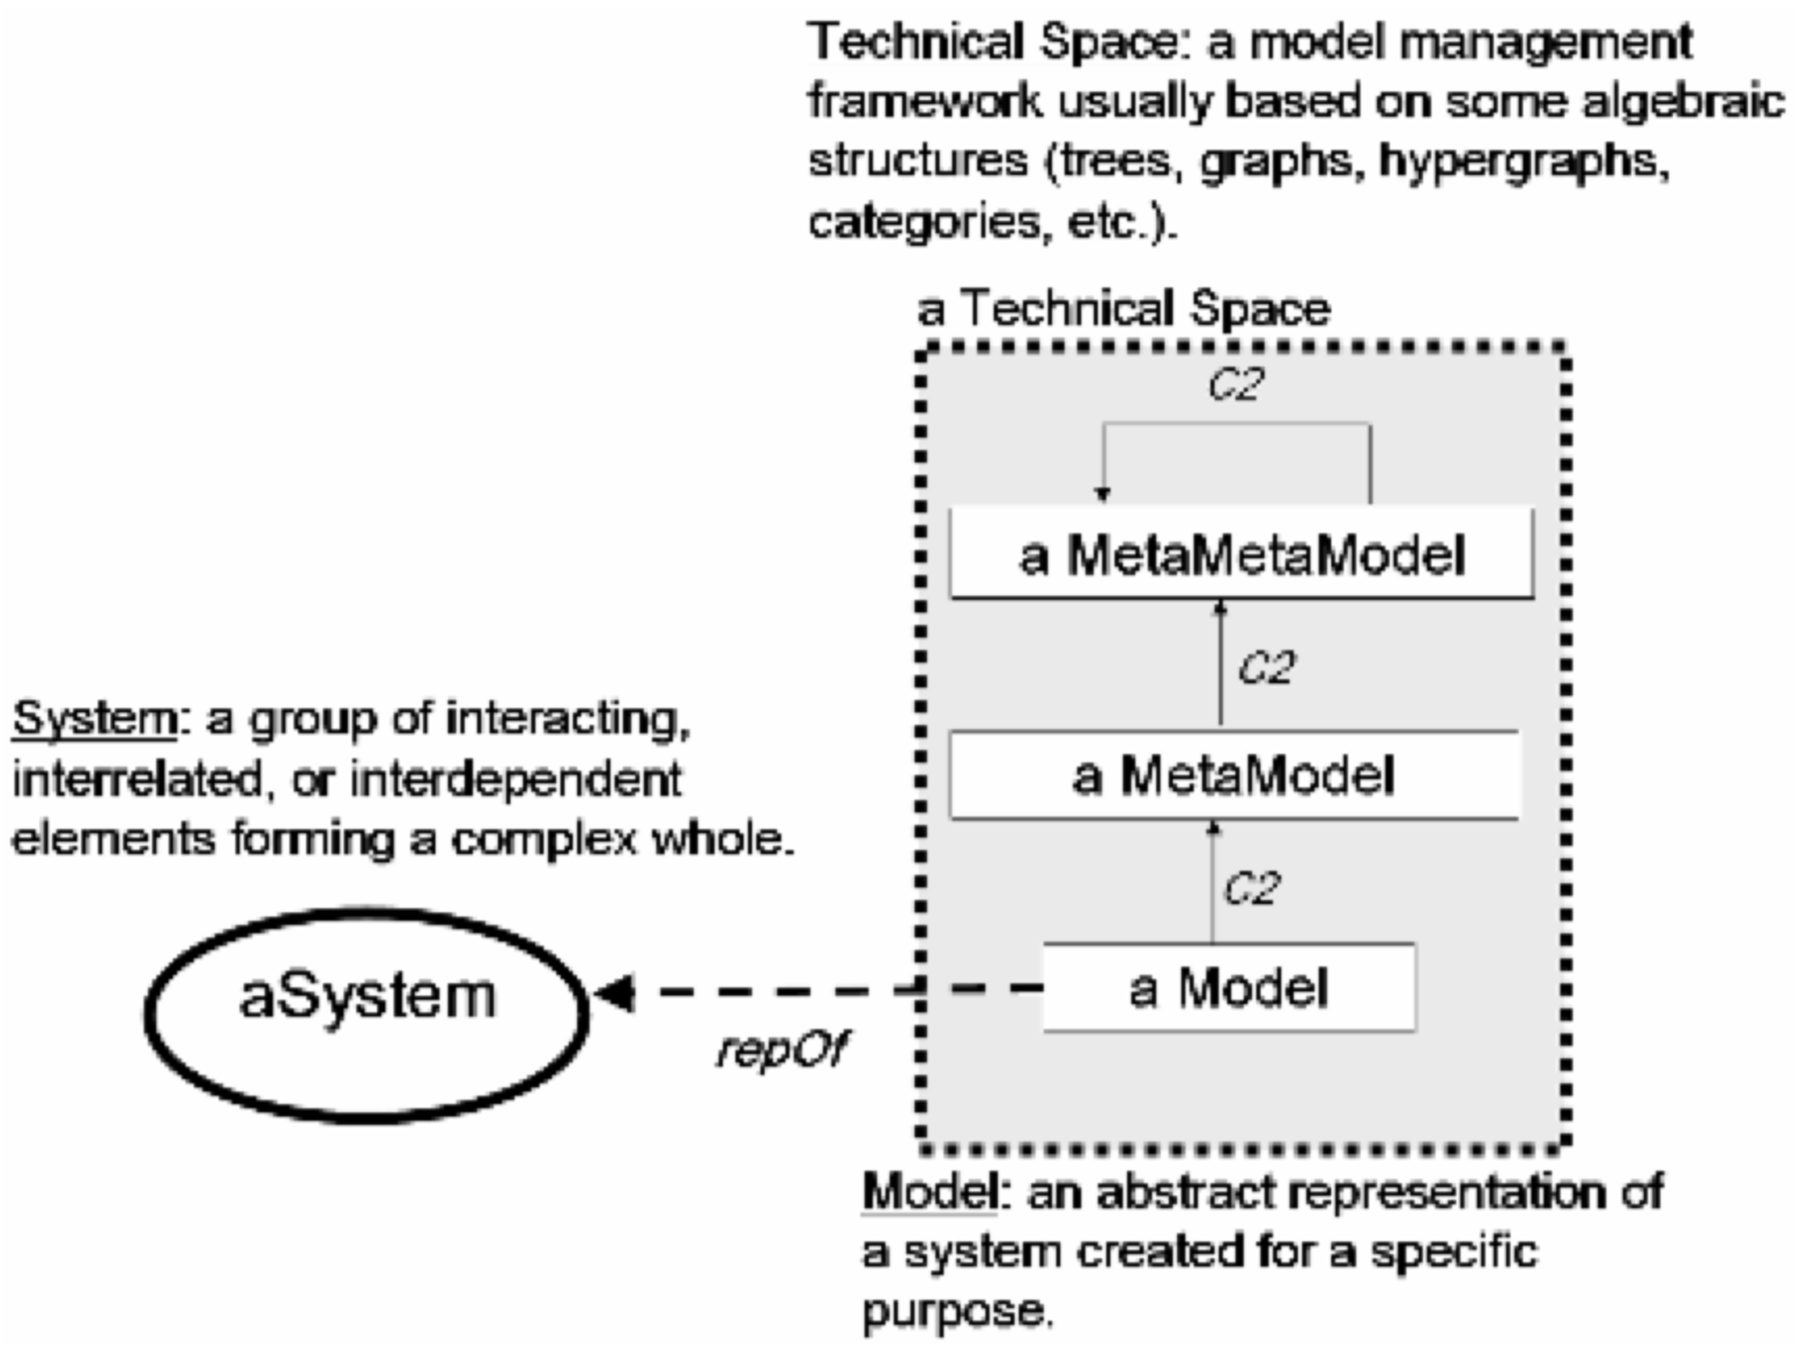
\includegraphics[width=0.6\textwidth]{images/dataset/bezivin2006_metamodel}
  \caption[An overview of systems, models and technical spaces]{Systems, models and technical spaces. (From \citep{Bezivin:2006gw}.)}
  \label{fig:dataset:bezivin2006_metamodel}
\end{figure}

We captured these concepts in a prototypical exploration process, first by developing a prototype system iteratively with a data tagging team who manually curated the data. Once this prototype was stable, we developed a model (\cref{sec:dataset:architecture:what_to_capture}) around the prototype. We generalised the system we had developed, expanding from a model we had designed that was marathon-specific, into a more generalisable metamodel (\cref{sec:dataset:architecture:metamodel}). We represent our process as as a \gls{uml} activity sequence diagram, shown in \cref{fig:dataset:methodology}.

The initial phase in our dataset development was to create a prototype system with the specific purpose of tagging our marathon runner context (using the dataset provided by the industry client). We name this partial implementation \textit{Argus}\footnoteurl{http://www.deakin.edu.au/~ca/argus}{5 July 2017}\footnote{Whose name is inspired by the \textit{all-seeing} giant of the same name from Greek mythology: ``With his multiple sets of eyes, Argus could see nearly everything in his vicinity''. See \url{http://www.loggia.com/myth/argus.html}.}. Refer to \cref{sec:dataset:argus} for more about this implementation. 

To develop this initial model (and thus to then what our metamodel would be), we began by discussing what requirements were needed---that is, the key features that we thought were necessary for extracting from our image. Five features were decided: (1) the crowdedness of the photo, (2) the visible bib sheets within the photo, (3) the faces corresponding to those bib sheets, (4) the prominence of runners of the photo and (5) the colours of runners' clothing in the photo.

Once an initial prototype was developed, we conducted informal usability tests with members from \gls{dstil}, which captured minor flaws in the workflow (namely required conditions that were missing in annotations) as well as general usability enhancements. Once the internal testing had concluded, we developed instructional video guides on how to use Argus, and then deployed the tool to a data tagging team that made the data available to us.

After deployment, we ran four iterations of tagging with our external data tagging team. We use the term \textit{iteration} to refer to the process of deploying Argus to the data tagging team, capturing a set of photos from various races, and sending the data back for quality assurance. These iterations consisted of photos from different marathon races in our dataset. (To ensure variance in tagging, there were some races at night and some races with alphanumeric components in the \gls{rbn}.) After each iteration we assessed the tagging for quality. Feedback identified further restrictions that needed to be placed on Argus as poor approximations or incorrect tagging would cause our \gls{ai} to learn poorly. 

The following issues were identified:

\begin{itemize}
  \item face region was too far away from the bib region,
  \item face region was overlapping the bib region,
  \item \glspl{rbn} had spaces,
  \item misidentified \glspl{rbn} where the alphabetic `I' was tagged as the numeric `1'.
\end{itemize}

\noindent
Furthermore, we added geometric restrictions and conditions into the tool to prevent these errors from occurring at all (i.e., ensuring faces could only be marked above and horizontally near bibs). Some of these issues are highlighted in \cref{fig:dataset:issues_with_tagging}.

\begin{figure}[p]
  \centering
  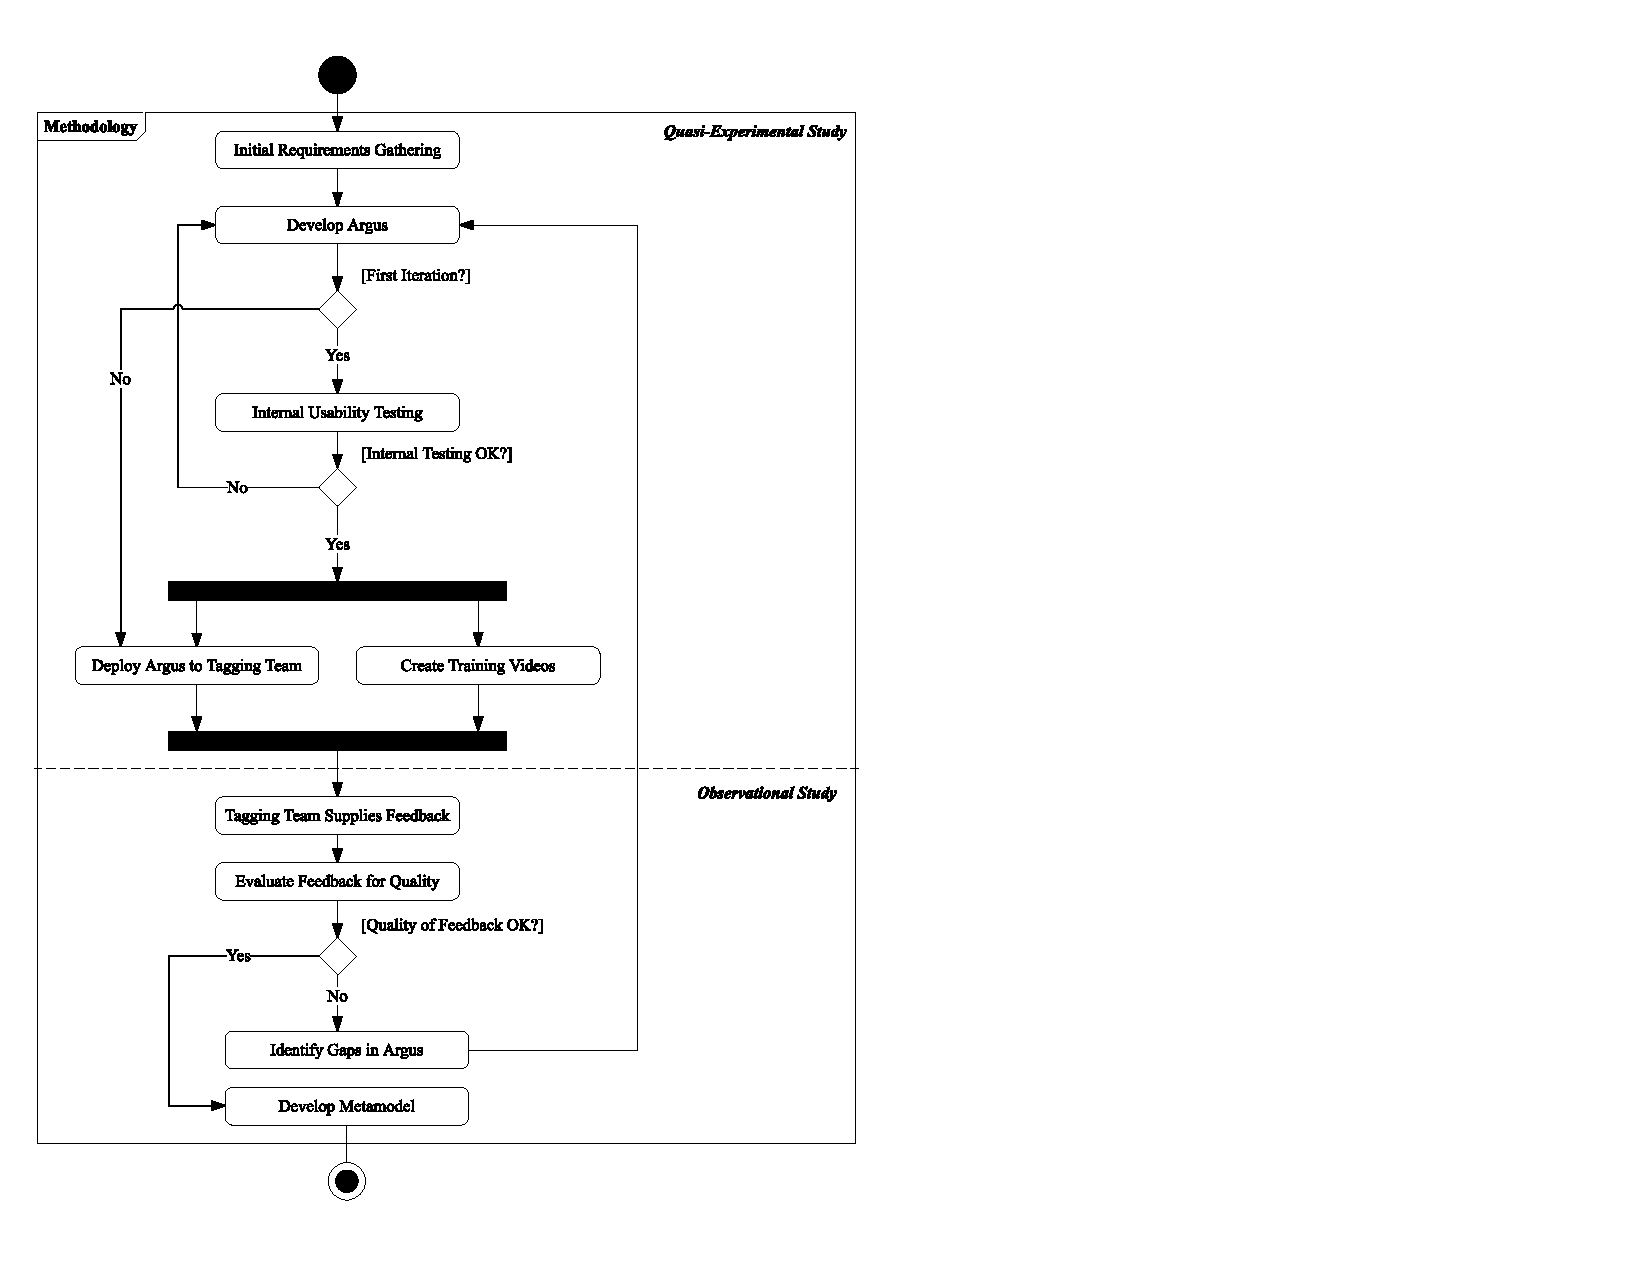
\includegraphics[width=0.7\textwidth]{images/dataset/methodology}
  \caption[Implementation methodology]{An overview of the methodology used to discover our metamodel.}
  \label{fig:dataset:methodology}
\end{figure}

\begin{figure}[p]
  \centering
  
  \begin{subfigure}[b]{0.8\textwidth}
    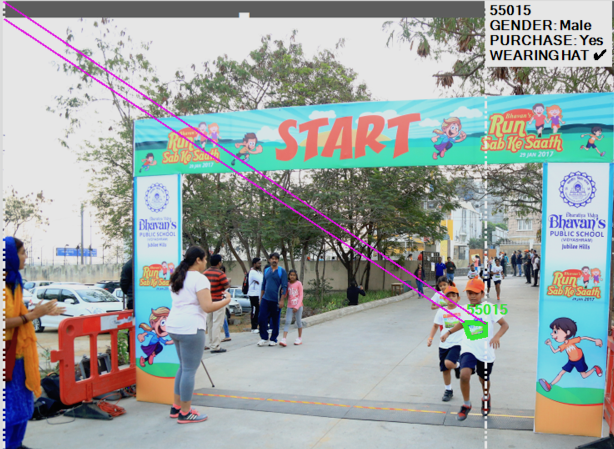
\includegraphics[width=\textwidth]{images/dataset/BadTagging_TooFar}
  \end{subfigure}\\
  \vspace{1cm}
  \hspace{\fill}
  \begin{subfigure}[b]{0.3\textwidth}
    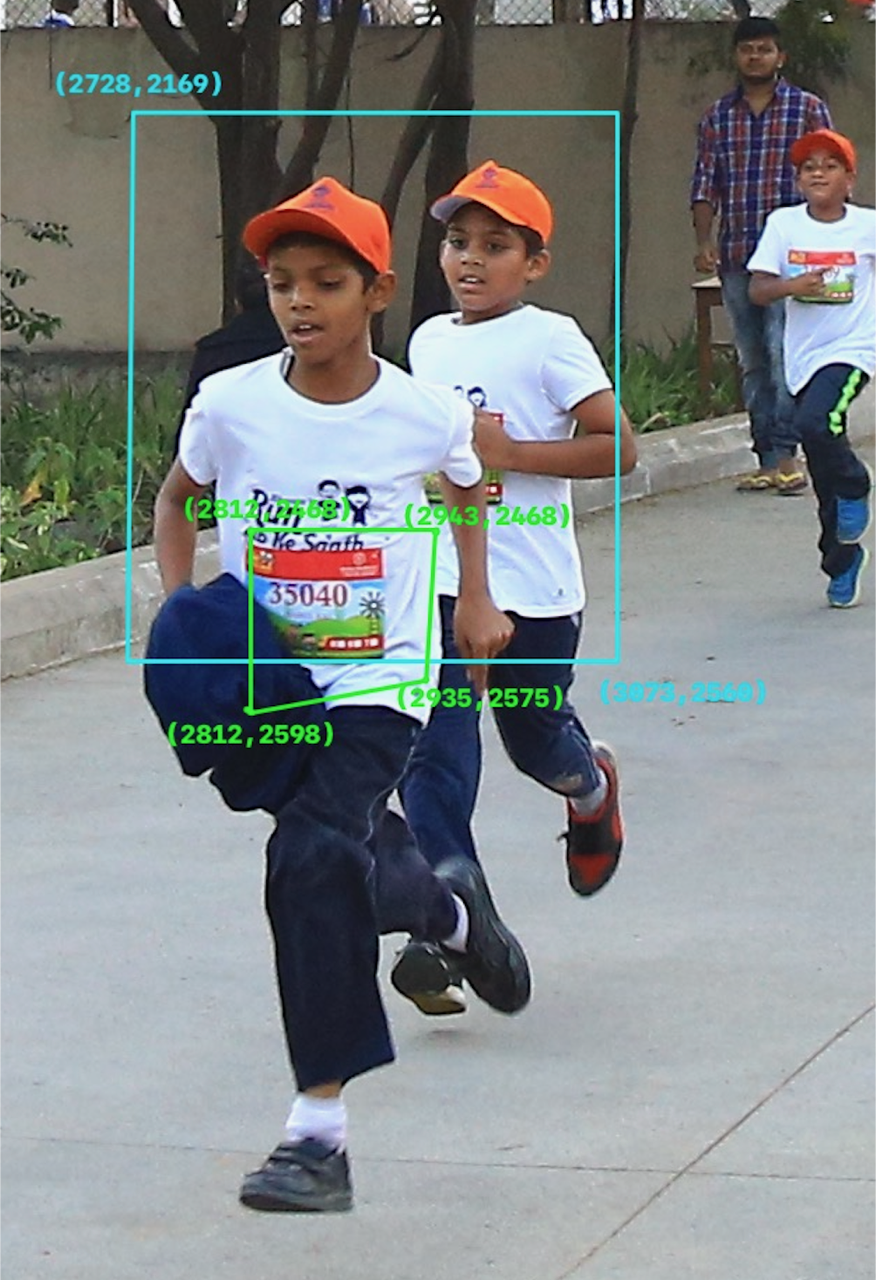
\includegraphics[width=\textwidth]{images/dataset/BadTagging_Overlap}
  \end{subfigure}
  \hspace{\fill}
  \begin{subfigure}[b]{0.3\textwidth}
    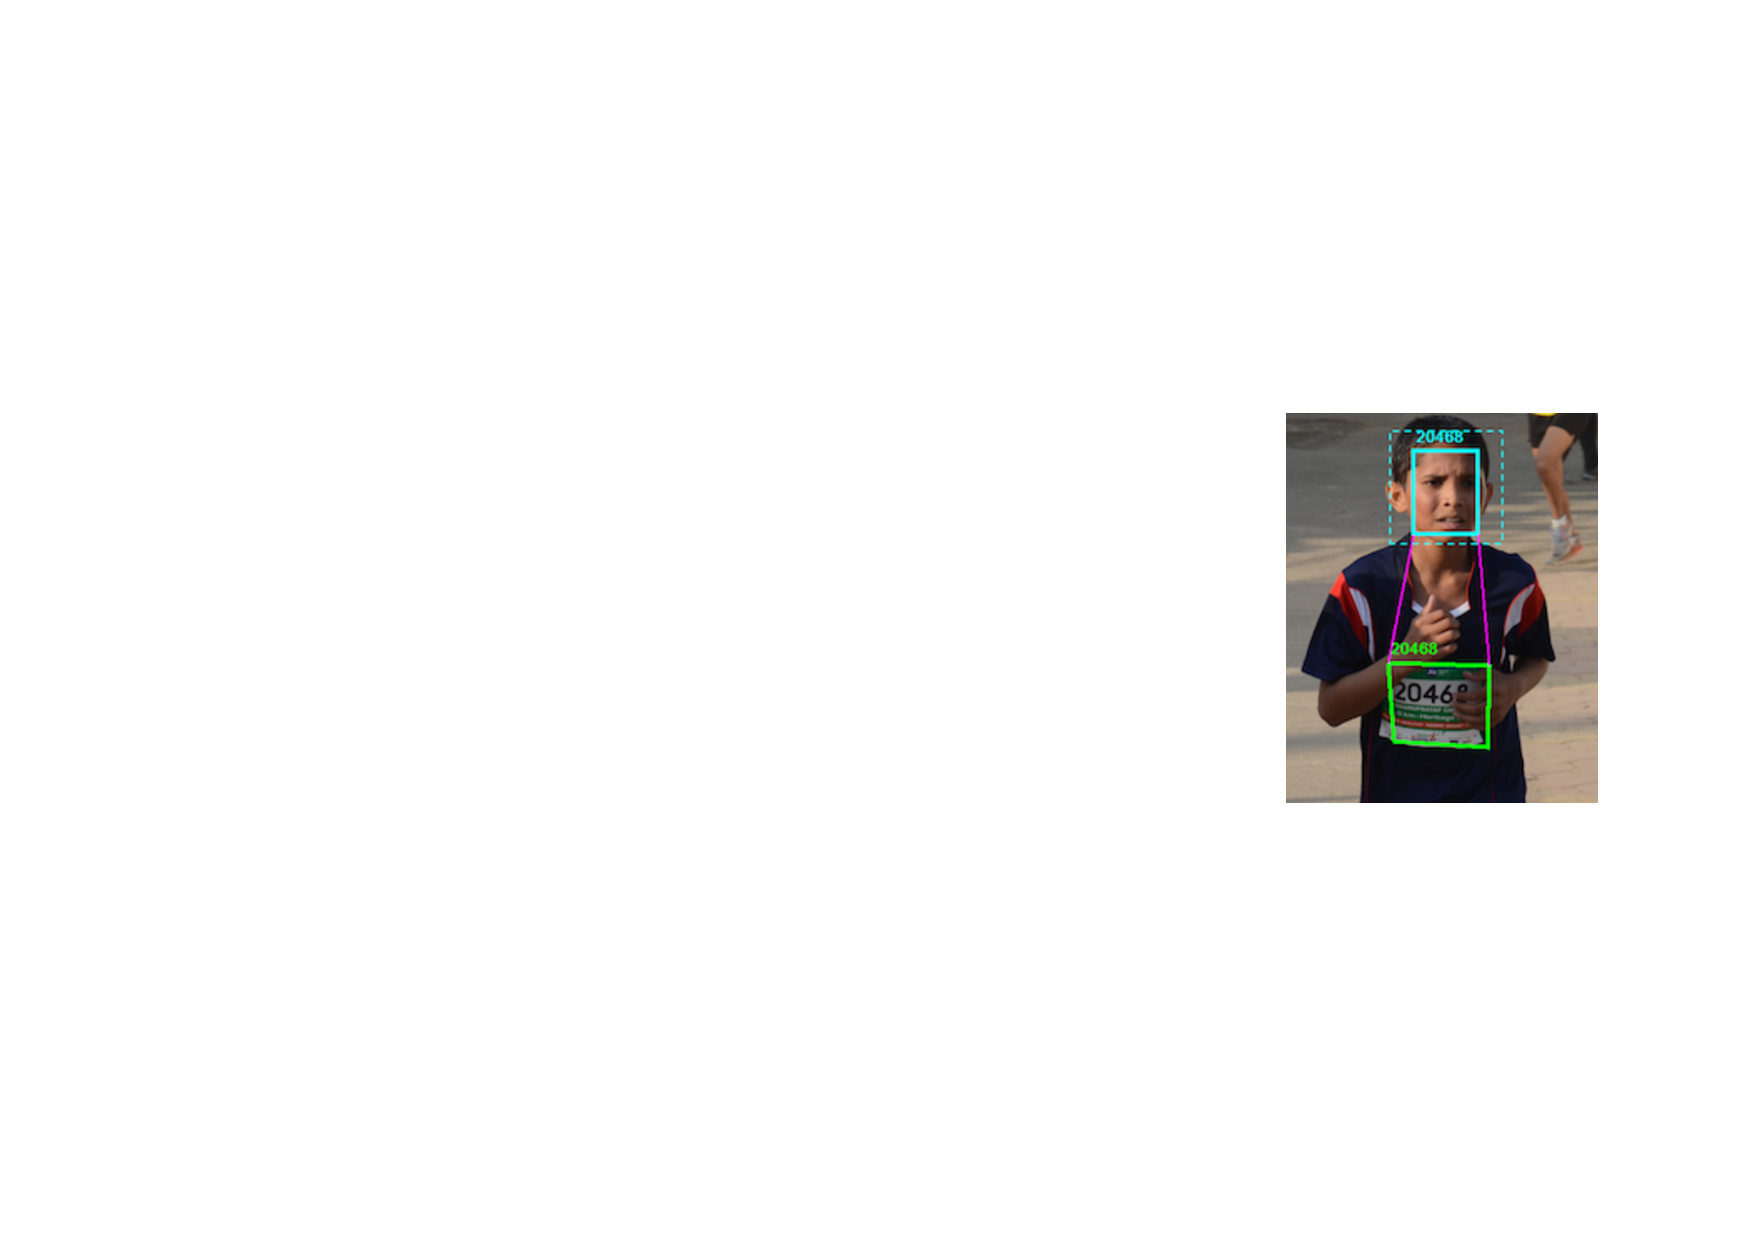
\includegraphics[width=\textwidth]{images/dataset/BadTagging_NotAroundFace}
  \end{subfigure}
  \hspace{\fill}  
  \begin{subfigure}[b]{0.2\textwidth}
    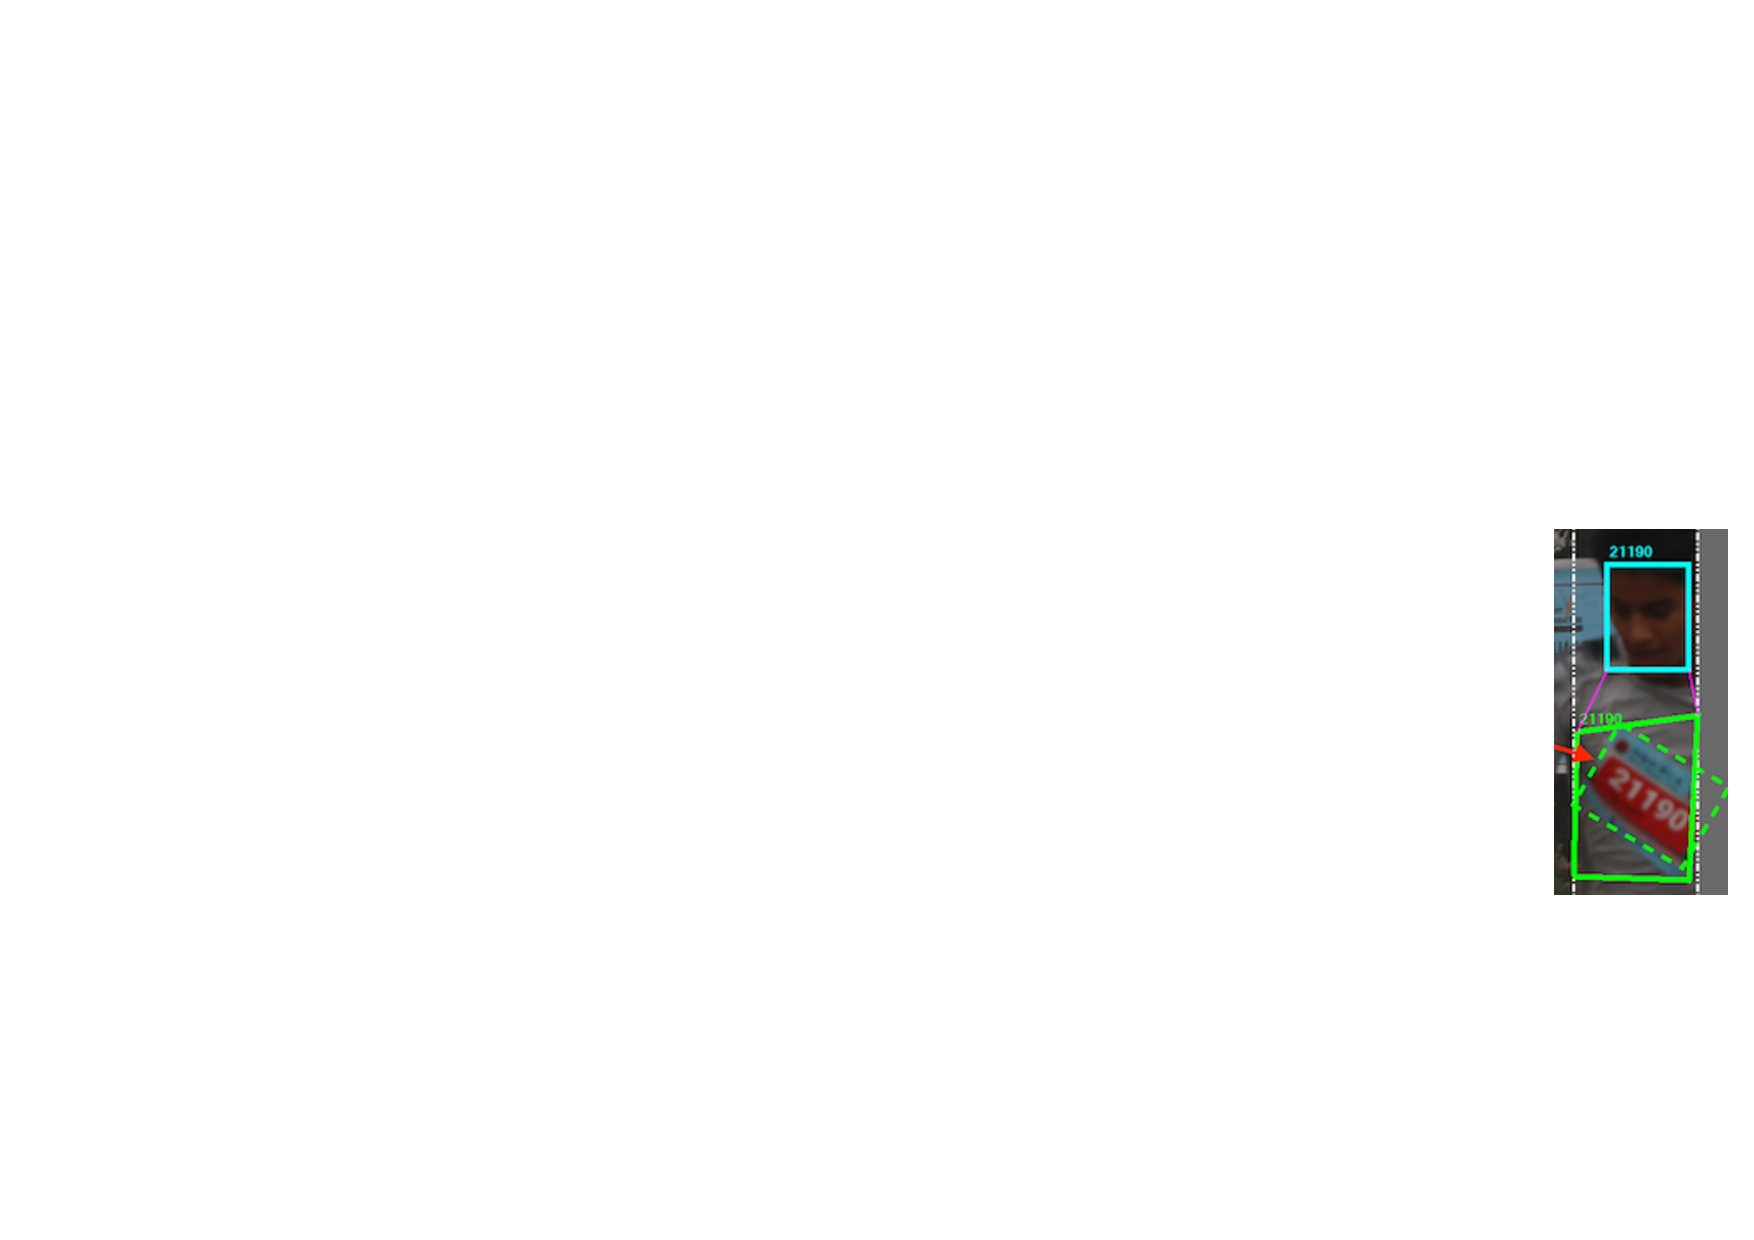
\includegraphics[width=\textwidth]{images/dataset/BadTagging_NotAroundBib}
  \end{subfigure}
  \hspace{\fill}
  
  \caption[Product testing issues identified]{Issues identified from rounds of external testing to the tagging team. Cyan lines indicate face regions, lime lines indicate bib regions, magenta lines indicate bib-to-face guidelines. \textit{Clockwise:} Face region is too far away from bib region; bib region is poorly marked (dotted lines expected); face region is too small (dotted lines expected); face region overlaps bib region.}
  \label{fig:dataset:issues_with_tagging}
\end{figure}

\section{Motivating Case Study: What to Capture?}
\label{sec:dataset:architecture:what_to_capture}

Let us consider the motivating case study of marathon races and determine the model of our dataset. What features do we want to capture from images within our dataset? To answer this question, we need to consider what information we see as relevant in a standard marathon photo (such as \cref{fig:introduction:background:sample_rbns}). We will consider five distinct features in the following sections.

\subsection{Feature 1: Image-Level Features}

There are two features to describe components of the entire photo that we call \textit{Image-level} features:

\begin{enumerate}
  \item whether or not the photo is considered as \textbf{crowded} (\textsc{true} or \textsc{false}), and
  \item an \textit{optional} collection of \textbf{runners} in the photo, given that the photo is not crowded.
\end{enumerate}

\begin{figure}[th]
  \centering
  \begin{subfigure}[b]{0.4\textwidth}
    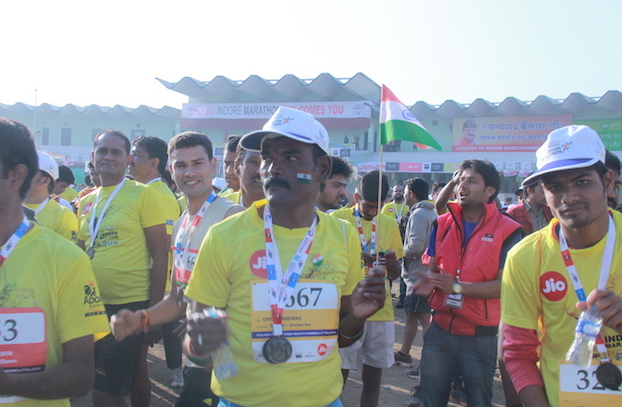
\includegraphics[width=\textwidth]{images/dataset/ImageFeatures_Crowded}
    \caption{\footnotesize A crowded photo.}
    \label{fig:dataset:image_features:crowded}
  \end{subfigure}
  \hspace{0.05\textwidth}
  \begin{subfigure}[b]{0.4\textwidth}
    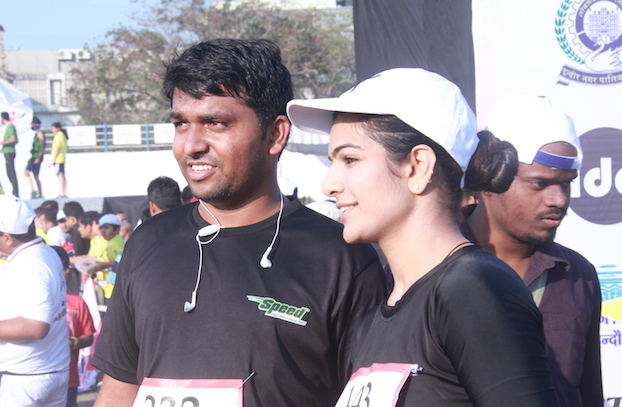
\includegraphics[width=\textwidth]{images/dataset/ImageFeatures_Optional_RBNsCropped}
    \caption{\footnotesize A photo where all \glspl{rbn} are cropped.}
    \label{fig:dataset:image_features:rbns_cropped}
  \end{subfigure}\\
  \vspace{1cm}
  \begin{subfigure}[b]{0.4\textwidth}
    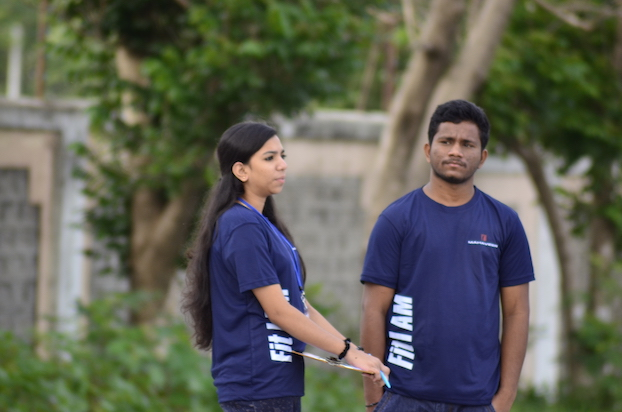
\includegraphics[width=\textwidth]{images/dataset/ImageFeatures_Optional_NoRBNs}
    \caption{\footnotesize A photo where there are no \glspl{rbn} present.}
    \label{fig:dataset:image_features:no_rbns}
  \end{subfigure} 
  \caption[Various image-level features]{Image-level features. In (a), the $PhotoCrowded$ annotation would be marked as \textsc{true}. Note the obstruction of all \glspl{rbn} in this photo. In (b) and (c), $PhotoCrowded$ is \textsc{false}, but there are no $Runners$ to tag.}
  \label{fig:dataset:image_features}
\end{figure}

We train a \gls{nn} based on photos that are not crowded; photos that are considered crowded are typically not desirable as runners prefer photos where they are the key subject. We therefore discard these photos to remove any potential bias tat the \gls{ai} could learn. We can only tag runners on the condition that the photo is not marked as crowded (\cref{fig:dataset:image_features:crowded}). Additionally, in some photos, all \glspl{rbn} are missing within the photo (e.g., hidden behind other runners, cropped out of view) and some photos contain no runners at all (\cref{fig:dataset:image_features:rbns_cropped,fig:dataset:image_features:no_rbns}). We therefore identify this as an \textit{optional} collection as we must associate an \gls{rbn} to a runner---the photo is not crowded, but there are no runners to tag, thereby making the annotation optional. Thus, an \textit{derived attribute} exists with such a collection: the \textit{count} of the runners in a photo is something we can automatically count.

\subsection{Feature 2: Bibs}

We identify the following two annotations of what we would label for a given runner's bib sheet. This is summarised in \cref{fig:dataset:bib_sheet_features}. Within this feature we identify the following annotations for \glspl{rbn}:

\begin{enumerate}
  \item a polygon around the runner's \textbf{bib sheet} that contains the $x$ and $y$ coordinates, given that there are exactly four vertices of this polygon
  \item a string with the runner's \textbf{\gls{rbn}}, once the bib sheet is tagged (exists).
\end{enumerate}

\begin{figure}[p]
  \centering
  \hspace{\fill}
  \begin{subfigure}[b]{0.25\textwidth}
    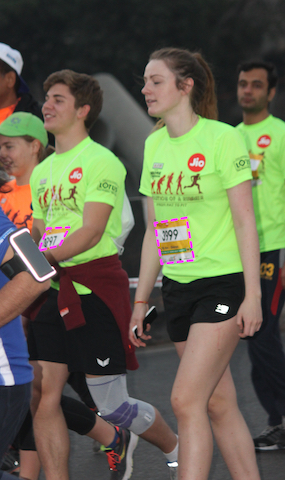
\includegraphics[width=\textwidth]{images/dataset/BibSheet_Detection}
  \end{subfigure}
  \hspace{\fill}
  \begin{subfigure}[b]{0.25\textwidth}
    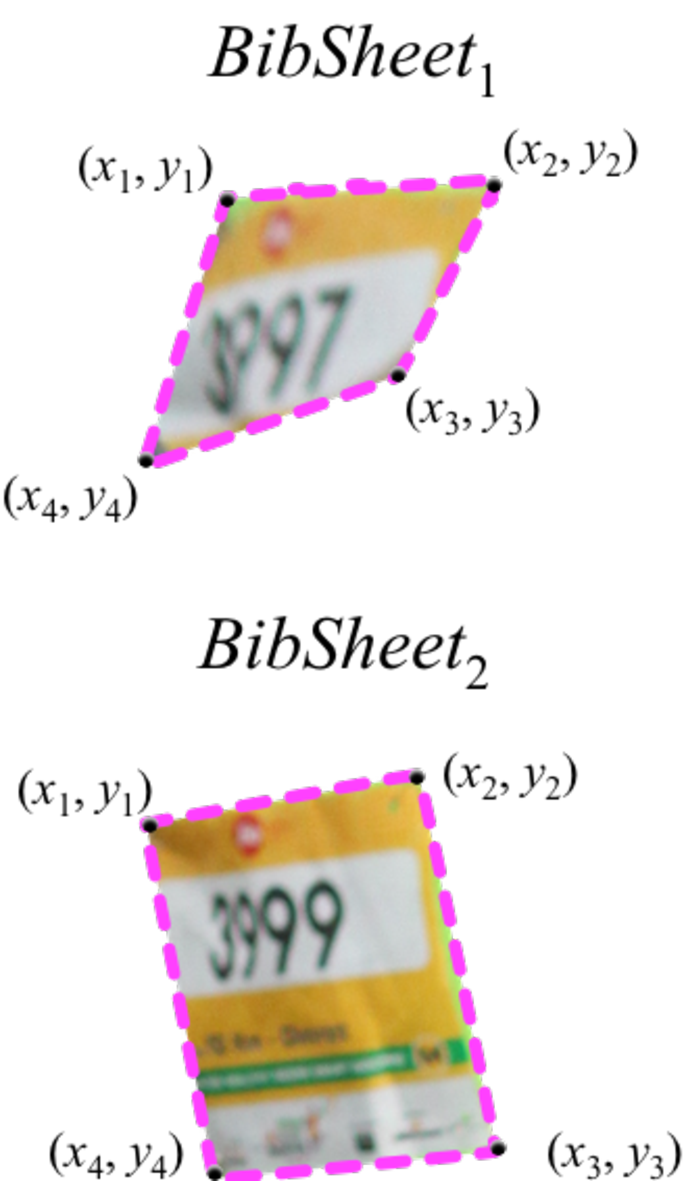
\includegraphics[width=\textwidth]{images/dataset/BibSheet_Area}
  \end{subfigure}
  \begin{subfigure}[b]{0.25\textwidth}
    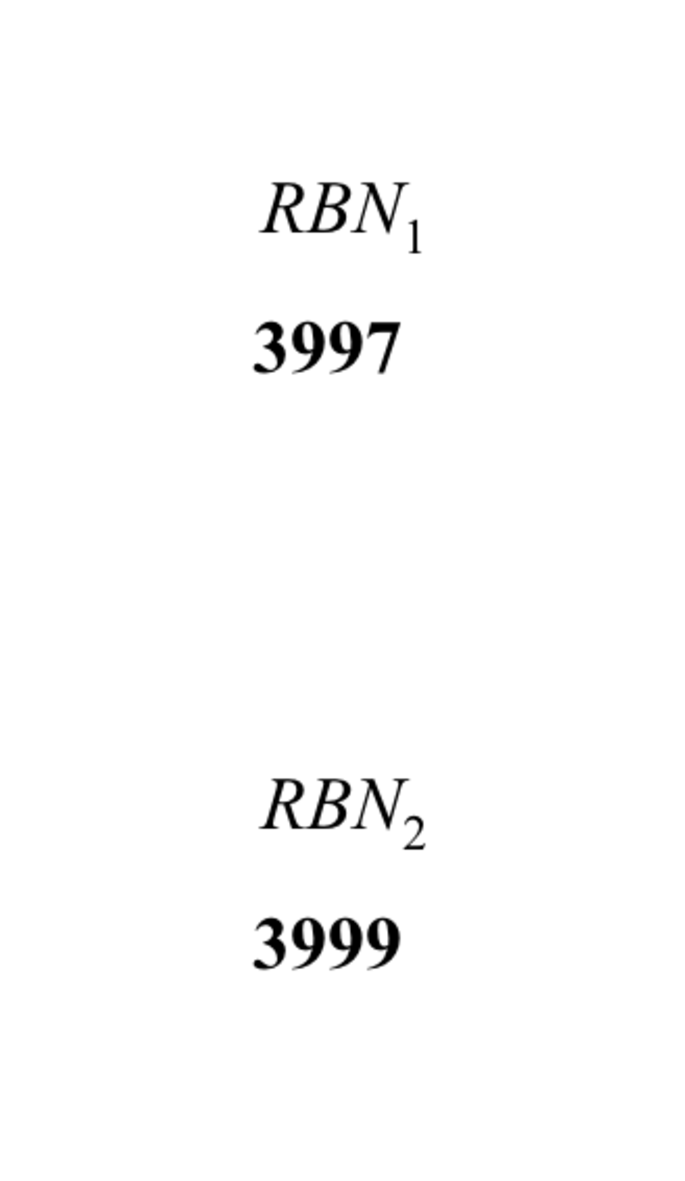
\includegraphics[width=\textwidth]{images/dataset/BibSheet_RBN}
  \end{subfigure} 
  \hspace{\fill}
  \caption[Bib Sheet segment-level features]{The bib segment-level feature. \textit{From left to right}: The manually annotated bib sheets in the original photo (outlined in magenta); the relative $BibSheet$ annotations with the four respective vertices; the detected $RBN$ input strings for the corresponding $BibSheet$.}
  \label{fig:dataset:bib_sheet_features}
\end{figure}

\subsection{Feature 3: Faces}

A further feature that is important is the runner's face region (\cref{fig:dataset:face_features}), which could compromise of five annotations:

\begin{enumerate}
  \item a rectangle around the runner's \textbf{face} that contains the two $x$ and $y$ coordinates of the two opposite vertices, given that the $bottom$ of this rectangle are above the $top$ of the bib sheet,
\end{enumerate}

\noindent
and once this face bounds has been tagged, more annotations can be extracted:

\begin{enumerate}
  \setcounter{enumi}{1}
  \item whether or not the runner is \textbf{wearing} a \textbf{hat} (\textsc{true} or \textsc{false}),
  \item whether or not the runner is \textbf{wearing} \textbf{(sun)glasses} (\textsc{true} or \textsc{false}), and
  \item the \textbf{gender} of the runner (\textsc{male}, \textsc{female}, or \textsc{unsure}).
\end{enumerate}

The bib sheet polygon would contain four \textit{explicit attributes} required as input by the tagger: the coordinates of its four vertices, $\{ (x_{1}, y_{1}), (x_{2}, y_{2}), (x_{3}, y_{3}), (x_{4}, y_{4}) \}$. Similarly, there are two explicit attributes required for the runner's face rectangle: the coordinates of the top left and the bottom right of the rectangle (i.e., the two opposite vertices) of the runner's face bounds, $\{ (x_{1}, y_{1}), (x_{2}, y_{2}) \}$. As both of these are shapes, we can automatically calculate the derived attributes from these coordinates:  $\{ top, left, bottom, right, width, height \}$.

\begin{figure}[p]
  \centering
  \hspace{\fill}
  \begin{subfigure}[b]{0.25\textwidth}
    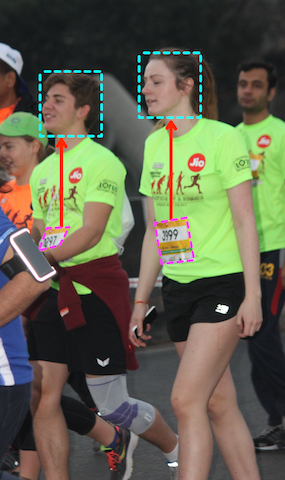
\includegraphics[width=\textwidth]{images/dataset/FaceBounds_Detection}
  \end{subfigure}
  \hspace{\fill}
  \begin{subfigure}[b]{0.25\textwidth}
    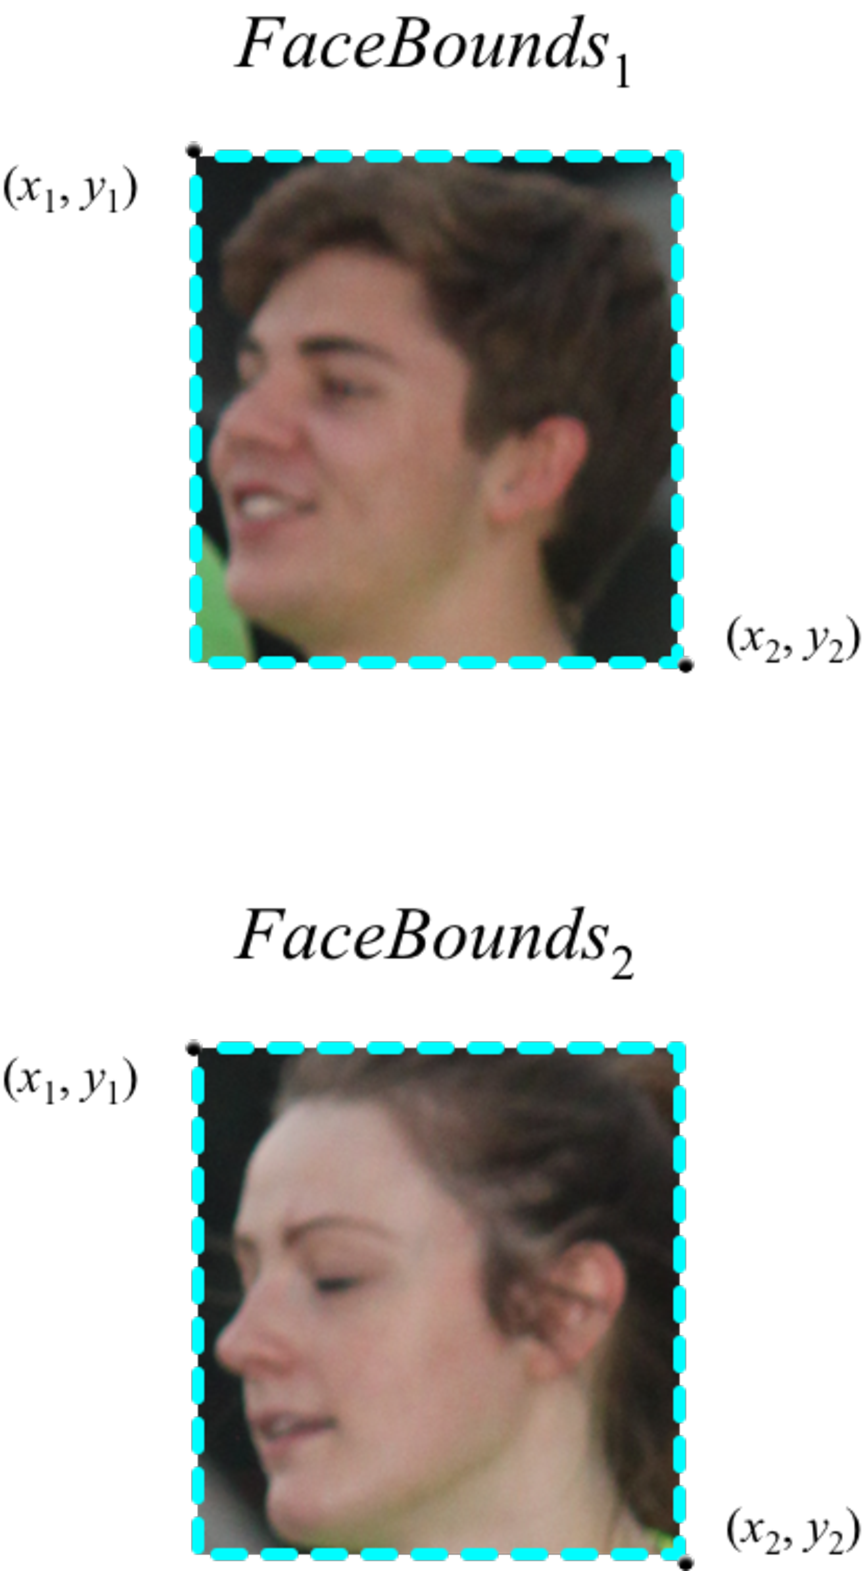
\includegraphics[width=\textwidth]{images/dataset/FaceBounds_Area}
  \end{subfigure}
  \hspace{\fill}
  \caption[Face Bounds segment-level features]{The face segment-level feature. \textit{Left}: The manually tagged face regions (cyan) that comply with the conditions that the bottom must be above the top of the bib (red arrows). \textit{Right}: the relative $FaceBounds$ annotations with the two opposite vertices. Other annotations in this feature would be: $WearingHat{1,2} = WearingGlasses{1,2} = \textsc{false}$, $Gender_{1} = \textsc{male}$, $Gender_{2} = \textsc{female}$.}
  \label{fig:dataset:face_features}
\end{figure}

%Given that the face region is tagged, we can then annotate:
%
%\begin{enumerate}
%  \item the `base classifications' of the person, and
%  \item the `colour classifications' of the person.
%\end{enumerate}

\subsection{Feature 4: Prominence}

We can now identify another feature, the prominence of the runner within the photo. These would consist of three annotations:

\begin{enumerate}
  \item whether or not the runner's \textbf{face} is \textbf{visible} (\textsc{true} or \textsc{false}),
  \item whether or not the runner is \textbf{blurry} (\textsc{true} or \textsc{false}),
  \item the \textbf{\gls{lop}} that the runner buys the photo (\textsc{no}, \textsc{maybe}, \textsc{yes}),
\end{enumerate}

A runner's face is considered `invisible' if it is obstructed by another object, cropped out of the image, or if the runner is looking down. See \cref{fig:dataset:face_prominence}. Runners are more likely purchase a photo if they are looking at the camera, and likewise if they are blurry in the image; these therefore have a significant impact on their prominence. We also define the \glsx{lop} value as a qualitative metric. We ask the data tagger to `picture' themselves as runner, and if so, we ask if they would purchase it. We then use this metric to train positive samples of good photos (\gls{lop} = \textsc{yes}) and samples of bad photos (\gls{lop} = \textsc{no}). Where \textsc{maybe} is provided, the runner is ignored to prevent training the network with indeterminate samples. Refer to \cref{fig:dataset:lop_prominence} for examples of the varying \gls{lop} values. 

\begin{figure}[p]
  \centering
  \hspace{\fill}
  \begin{subfigure}[b]{0.25\textwidth}
    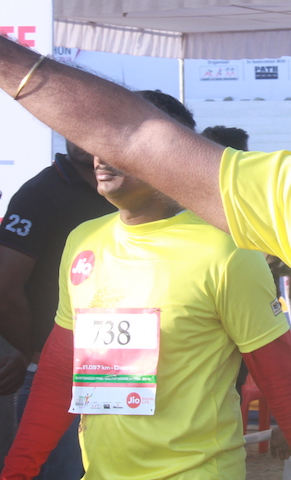
\includegraphics[width=\textwidth]{images/dataset/Prominence_FaceNotVisible_Covered}
    \caption{Face obstructed}
  \end{subfigure}
  \hspace{\fill}
  \begin{subfigure}[b]{0.25\textwidth}
    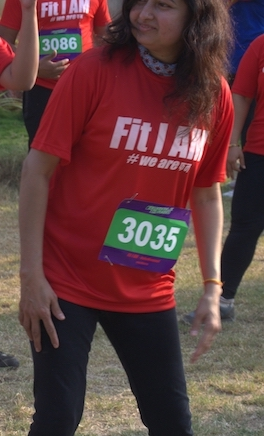
\includegraphics[width=\textwidth]{images/dataset/Prominence_FaceNotVisible_Cropped}
      \caption{Face cropped}
  \end{subfigure}
  \hspace{\fill}
  \begin{subfigure}[b]{0.25\textwidth}
    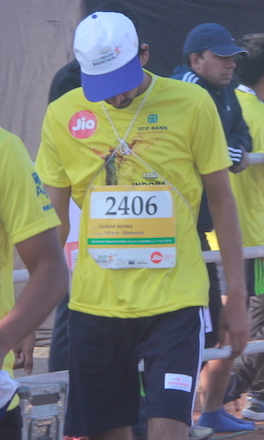
\includegraphics[width=\textwidth]{images/dataset/Prominence_FaceNotVisible_LookingDown}
    \caption{Face looking down}
  \end{subfigure}
  \hspace{\fill}
  \caption[Face visibility and its effect on prominence]{The $FaceVisible$ plays a significant impact on the prominence feature. Above are cases where the face would be marked as not visible.}
  \label{fig:dataset:face_prominence}
\end{figure}

\begin{figure}[p]
  \centering
  \hspace{\fill}
  \begin{subfigure}[b]{0.25\textwidth}
    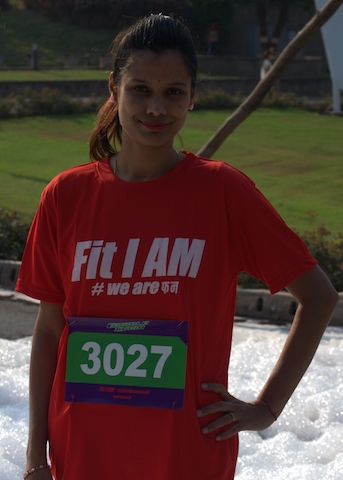
\includegraphics[width=\textwidth]{images/dataset/Prominence_LoP_Yes}
    \caption{\gls{lop} = \textsc{yes}}
  \end{subfigure}
  \hspace{\fill}
  \begin{subfigure}[b]{0.25\textwidth}
    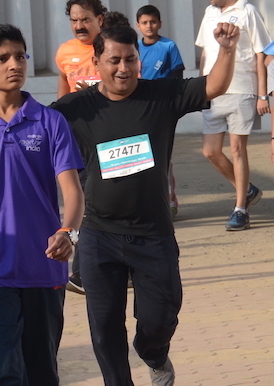
\includegraphics[width=\textwidth]{images/dataset/Prominence_LoP_Maybe}
    \caption{\gls{lop} = \textsc{maybe}}
  \end{subfigure}
  \hspace{\fill}
  \begin{subfigure}[b]{0.25\textwidth}
    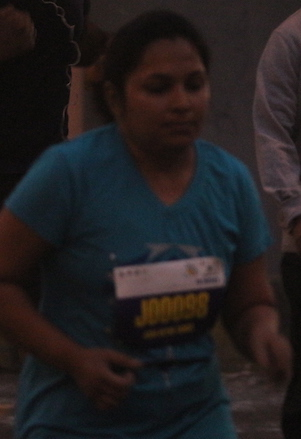
\includegraphics[width=\textwidth]{images/dataset/Prominence_LoP_No}
    \caption{\gls{lop} = \textsc{no}}
  \end{subfigure}
  \hspace{\fill}
  \caption[Variant Purchase Likelihoods]{Various examples of the $\gls{lop}$ values. In (a), the woman is clearly posing and is the primary subject of the photo. In (b), the runner is in focus in a pose, but is behind another runner and there are other runners behind him. In (c), the woman is out of focus, is blurry, and this photo has very poor lighting conditions.}
  \label{fig:dataset:lop_prominence}
\end{figure}

\subsection{Feature 5: Colours}

Another feature we can capture is a way to identify runners by the colour of their clothing. (Within our dataset, various clothing items of distinct colours are given to runners for particular races.) These features comprise of four annotations:

\begin{enumerate}
  \item an \textit{optional} \textbf{colour} of the runner's \textbf{hat}, given that they were annotated as wearing a hat,
  \item the \textbf{colour} of the runner's \textbf{shirt},
  \item an \textit{optional} \textbf{colour} of the runner's \textbf{shorts}, and
  \item an \textit{optional} \textbf{colour} of the runner's \textbf{shoes}.
\end{enumerate}

% TODO: Example of colour matching. Do we capture the coordinates?

The colour of a runner's shirt is required, as we expect that a bib would be detected on the shirt of a runner (which would be tagged). The other colour annotations are all optional, as it is likely that some of these clothing items may be cropped out of the photo or is not visible. Furthermore, the hat colour can only be specified on the condition that the tagger has marked the runner has wearing a hat.

We can segment groups of the annotations we extract into features of two categories: annotations that feature at the \textit{image}-level and those that do not, which we call \textit{segment}-level features. The image-level features are those which apply to the entire image (i.e., $PhotoCrowded$, $Runners$). Those that apply at the segment level can be grouped into what types of features we are extracting: the runner's bib, face, their prominence and their colour identification.

In summary, we have identified a total of 5 features of 15 annotations, which are summarised within \cref{tab:dataset:annotation_summary}. Each of these annotations can be classified with a name and type, conditions for the annotation to be valid, dependencies on other annotations to exist before the annotation can be made, explicit attributes which the tagger must specify, derived attributes which we can automatically compute, possible values which limit the range of data for that annotation, and whether or not the annotation is optional.

\begin{landscape}

\begin{table}[p]
  \centering
  \caption[Summary of annotations captured in the dataset]{\centering A summary of the annotations we wish to capture from our dataset. Image and segment-level features are separated using the double line.}
  \label{tab:dataset:annotation_summary}
  \tablefitlandscape{
    \begin{tabular}{llllllllll}
      \toprule
        \textbf{Feature} &
        \textbf{Annotation} &
        \textbf{Type} &
        \textbf{Conditions} &
        \textbf{Dependencies} &
        \textbf{Explicit Attributes} &
        \textbf{Derived Attributes} &
        \textbf{Possible Values} &
        \textbf{Default} &
        \textbf{Optional}
      \\
      \midrule
        \multirow{2}{*}{Image-Level} &
        $PhotoCrowded$ &
        Boolean &
        N/A &
        N/A &
        N/A &
        N/A &
        $\{ \textsc{true}, \textsc{false} \}$&
        \textsc{false} &
        No
      \\
        &
        $Runners$ &
        Collection &
        $\{ PhotoCrowded = \textsc{false} \}$ &
        N/A &
        N/A &
        $\{count\}$ &
        N/A &
        \textsc{null} &
        Yes
      \\
      \midrule
      \midrule
        \multirow{2}{*}{Bib} &
        $BibSheet$ &
        Polygon &
        $\{ vertices = 4 \}$ &
        N/A &
        $\{ x_{1} \dots x_{4}, y_{1} \dots y_{4} \}$ &
        $\{ top, left, bottom, right, width, height \}$ &
        N/A &
        \textsc{null} &
        No
      \\
        &
        $\gls{rbn}$ &
        Label &
        N/A &
        $BibSheet$ &
        N/A &
        N/A &
        N/A &
        \textsc{null} &
        No
      \\
      \midrule
        \multirow{2}{*}{Face} &
        $FaceBounds$ &
        Rectangle &
        $\{ bottom > BibSheet_{top} \}$  &
        $BibSheet$ &
        $\{ x_{1}, y_{1}, x_{2}, y_{2}\}$ &
        $\{ top, left, bottom, right, width, height \}$ &
        N/A &
        \textsc{null} &
        No
      \\
        &
        $WearingHat$ &
        Boolean &
        N/A &
        $FaceBounds$ &
        N/A &
        N/A &
        $\{ \textsc{true}, \textsc{false} \}$&
        \textsc{false} &
        No
      \\
        &
        $WearingGlasses$ &
        Boolean &
        N/A &
        $FaceBounds$ &
        N/A &
        N/A &
        $\{ \textsc{true}, \textsc{false} \}$&
        \textsc{false} &
        No
      \\
        &
        $Gender$ &
        Category &
        N/A &
        $FaceBounds$ &
        N/A &
        N/A &
        $\{ \textsc{male}, \textsc{female}, \textsc{unsure} \} $ &
        \textsc{male} &
        No
      \\
      \midrule
        \multirow{2}{*}{Prominence} &
        $\gls{lop}$ &
        Category &
        N/A &
        $FaceBounds$ &
        N/A &
        N/A &
        $\{ \textsc{no}, \textsc{maybe}, \textsc{yes} \}$ &
        \textsc{maybe} &
        No
      \\
        &
        $FaceVisible$ &
        Boolean &
        N/A &
        $FaceBounds$ &
        N/A &
        N/A &
        $\{ \textsc{true}, \textsc{false} \}$&
        \textsc{true} &
        No
      \\
        &
        $Blurry$ &
        Boolean &
        N/A &
        $FaceBounds$ &
        N/A &
        N/A &
        $\{ \textsc{true}, \textsc{false} \}$&
        \textsc{false} &
        No
      \\
      \midrule
        \multirow{2}{*}{Colours} &
        $ShirtColor$ &
        Color &
        N/A &
        $FaceBounds$ &
        $\{ red, green, blue \}$ &
        N/A &
        N/A &
        \textsc{null} &
        No
      \\
        &
        $ShoeColor$ &
        Color &
        N/A &
        $FaceBounds$ &
        $\{ red, green, blue \}$ &
        N/A &
        N/A &
        \textsc{null} &
        Yes
      \\
        &
        $ShortsColor$ &
        Color &
        N/A &
        $FaceBounds$ &
        $\{ red, green, blue \}$ &
        N/A &
        N/A &
        \textsc{null} &
        Yes
      \\
        &
        $HatColor$ &
        Color &
        $\{ WearingHat = \textsc{true} \}$ &
        $FaceBounds$ &
        $\{ red, green, blue \}$ &
        N/A &
        N/A &
        \textsc{null} &
        Yes
      \\
      \bottomrule
    \end{tabular}
  }
\end{table}

\end{landscape}

% Run through an example of what it is we need to capture for our study & why (Refer to meeting 1 notes).
% state diagram of things we need to classify (break down diagram).

\section{Describing the Metamodel}
\label{sec:dataset:architecture:metamodel}

% Conceptualise what we have in our workflow as a meta model.
% What are the components, and constraints? Discuss why we needed to add in constraints... Feedback from India

In the example given in \cref{tab:dataset:annotation_summary}, we describe a model which was derived using information discovered from Argus' incremental development. In this section, we generalise this information and develop a metamodel . This metamodel is represented as a \gls{uml} class diagram, shown in \cref{fig:dataset:metamodel_class_diagram}.

\begin{figure}[h]
  \centering
  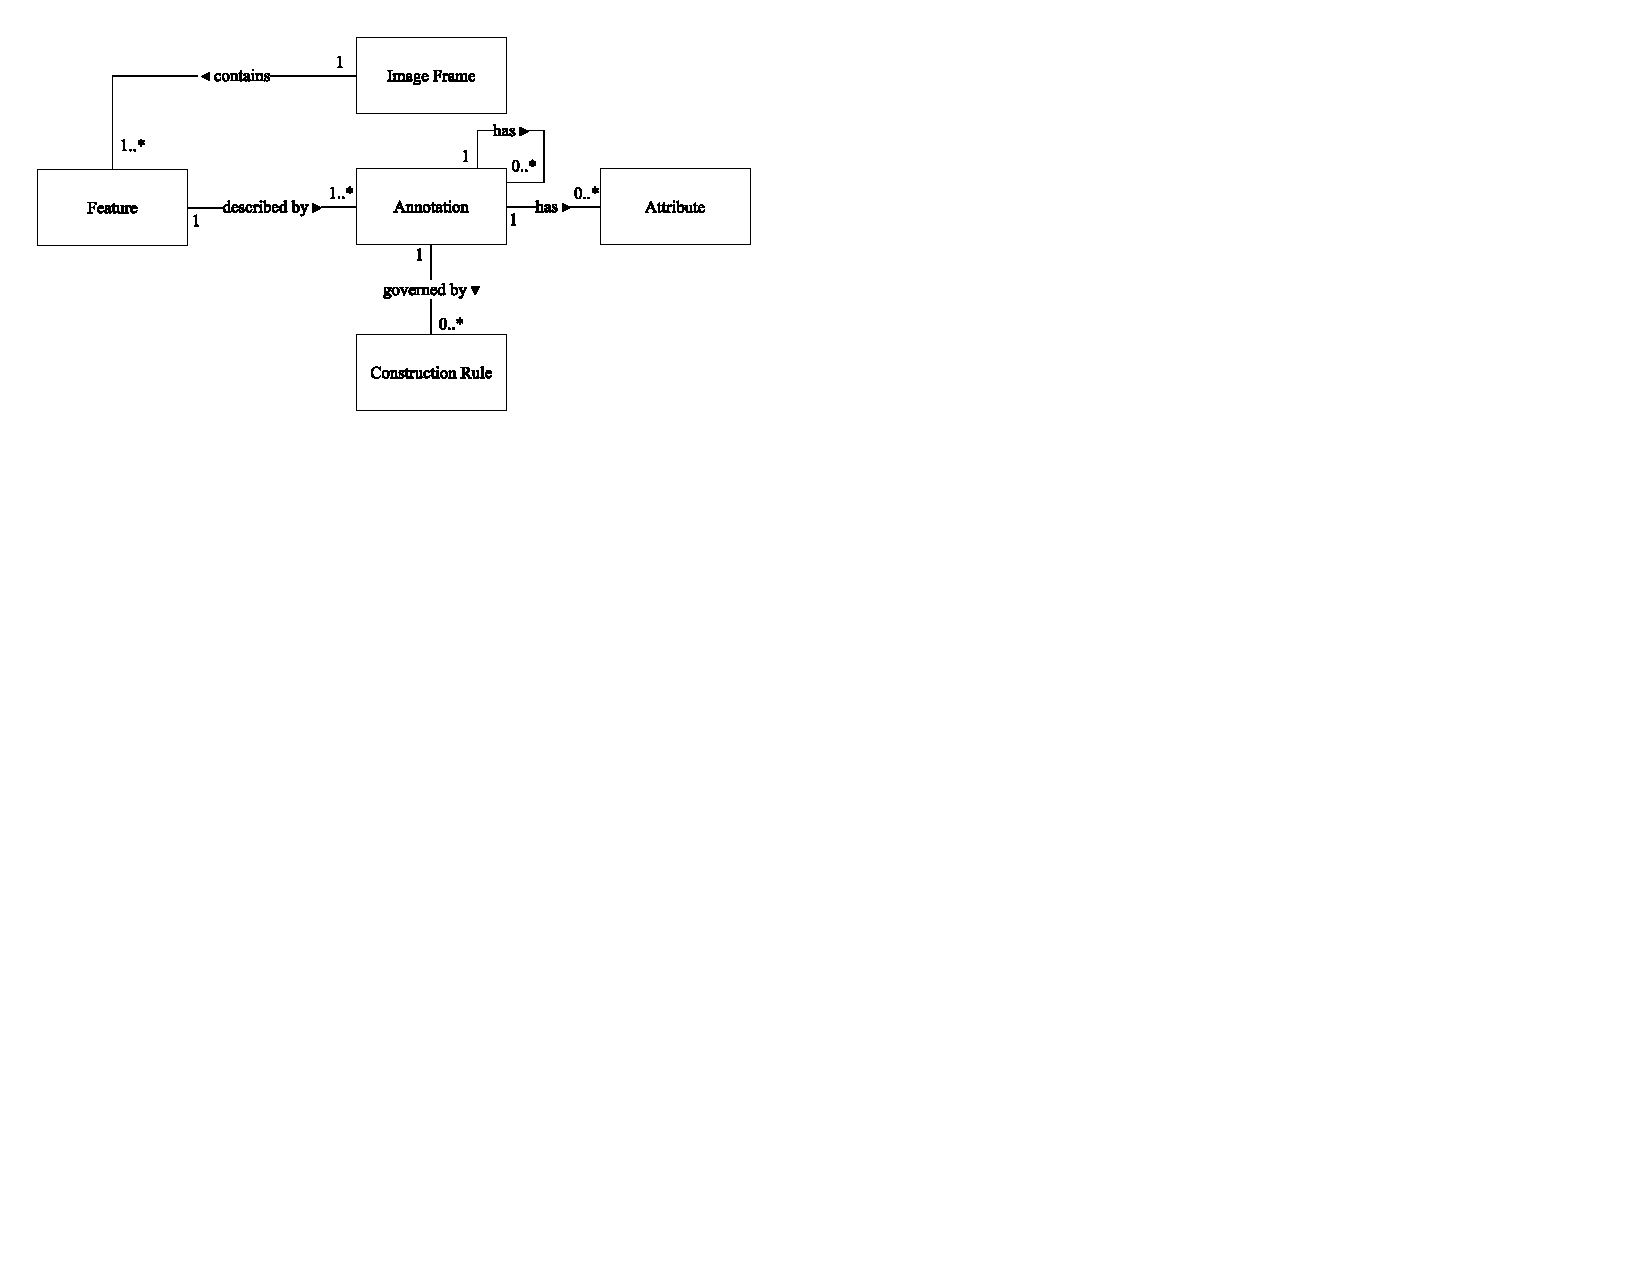
\includegraphics[width=\textwidth]{images/dataset/metamodel_class_diagram}
  \caption[Class diagram of our proposed metamodel]{A class diagram of our proposed metamodel.}
  \label{fig:dataset:metamodel_class_diagram}
\end{figure}

The core concept of this metamodel is an \textit{Annotation}, which (collectively) describe a feature within an image. Annotations may contain additional attributes to further extend what information they contain, and are governed by a set constrictions that we call \textit{Construction Rules}.

These form layers of data within images that we annotate, which can be represented in a hierarchical data format (e.g., a tree) that describes the layering of a fully annotated photo's features. These classes have further depth that are captured via inheritance models, presented in \cref{ch:metamodel_class_diagrams}.

We describe each of these classes in the following sections.

\subsection{Image Frame}

An image frame is any visual representation of a graphic. We extend the possibilities of our metamodel beyond just static images---these frames may be those found in videos also.

\subsection{Feature}

Image frames contain a certain number of features. These features are the key `concepts' within the image that we want to capture. There are two main features: (1) image-level features, and (2) segment-level features. Image-level features are those that apply to the entire frame and do not exist in a broken down context---we can't break down these features into their own subjects. This contrasts to segment-level features, which are features that only apply to a segmented region of the image. We identified four segment-level features in our example (all of which relate to one runner): Bib, Face, Prominence and Colours.

\subsection{Annotation}

Annotations are a set of feature descriptors that describes what the feature is compromised of. From \cref{tab:dataset:annotation_summary}, we describe a simple type system consisting of the following: \textit{Boolean}s, a restricted form of the \textit{Category} type (where possible values are $\{ \textsc{true}, \textsc{false} \}$); \textit{Polygon}s and \textit{Rectangle}s, generalised into a high-level \textit{Boundary} type; and \textit{Colour}s, represented as an RGB represented hexadecimal \textit{Label} (a generic labelling type). This only leaves our \textit{Collection} of runners: a data type which encompasses multiple annotations. Attributes can therefore be described by a type system that is generalisable from \textit{Labels}, \textit{Boundaries}, \textit{Collections} and \textit{Categories}. We model this as a type tree (\cref{fig:metamodel_class_diagrams:annotation}).

\subsection{Construction Rules} 

Construction Rules govern how attributes can be made. We break these down into four types: Dependencies, Conditions, Optionality and Restrictions (\cref{fig:metamodel_class_diagrams:construction_rules}). Some annotations are dependent on others existing---these are rules that we name \textit{Dependencies}. For instance, we cannot annotate an \gls{rbn} if there is no $BibSheet$ annotated. Likewise, a $FaceBounds$ is dependent on where the $BibSheet$ is, and so the $BibSheet$ must be marked up first. These dependencies add order in which features are being extracted, which is important to the tagger marking up the photo. A \textit{Condition} is a construction rule that disallows a data tagger to create an annotation until a condition is met by the annotator. For instance, we can never have a $BibSheet$ above a $FaceBounds$, so when we can specify this as a condition. These are not bound to just geometric constraints; we also see that we cannot tag $Runners$ if the $PhotoCrowded$ annotation is marked as \textsc{true}. Not all annotations are needed---in these cases the annotation is restricted by an \textit{Optional} construction rule; by default, all annotations are required, but we can specify these to be optional using such a rule. Lastly, \textit{Restrictions} exist to prevent invalid data from being tagged. In our example, we implemented two restrictions in Argus: (1) a face region must be tagged within an aspect ratio of $3 \times BibSheet_{width} : 5 \times BibSheet_{height}$, and (2) the opposite edges of a face region must be at least 15 pixels apart. This helps prevent issues shown in \cref{fig:dataset:issues_with_tagging}.

\begin{figure}[p]
  \centering
  
  \begin{subfigure}[b]{0.8\textwidth}
    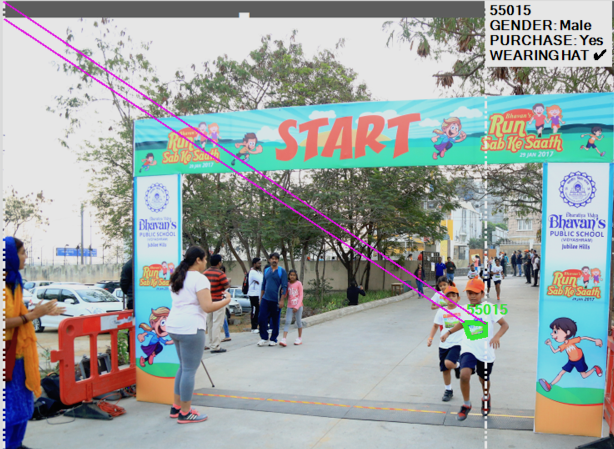
\includegraphics[width=\textwidth]{images/dataset/BadTagging_TooFar}
  \end{subfigure}\\
  \vspace{1cm}
  \hspace{\fill}
  \begin{subfigure}[b]{0.3\textwidth}
    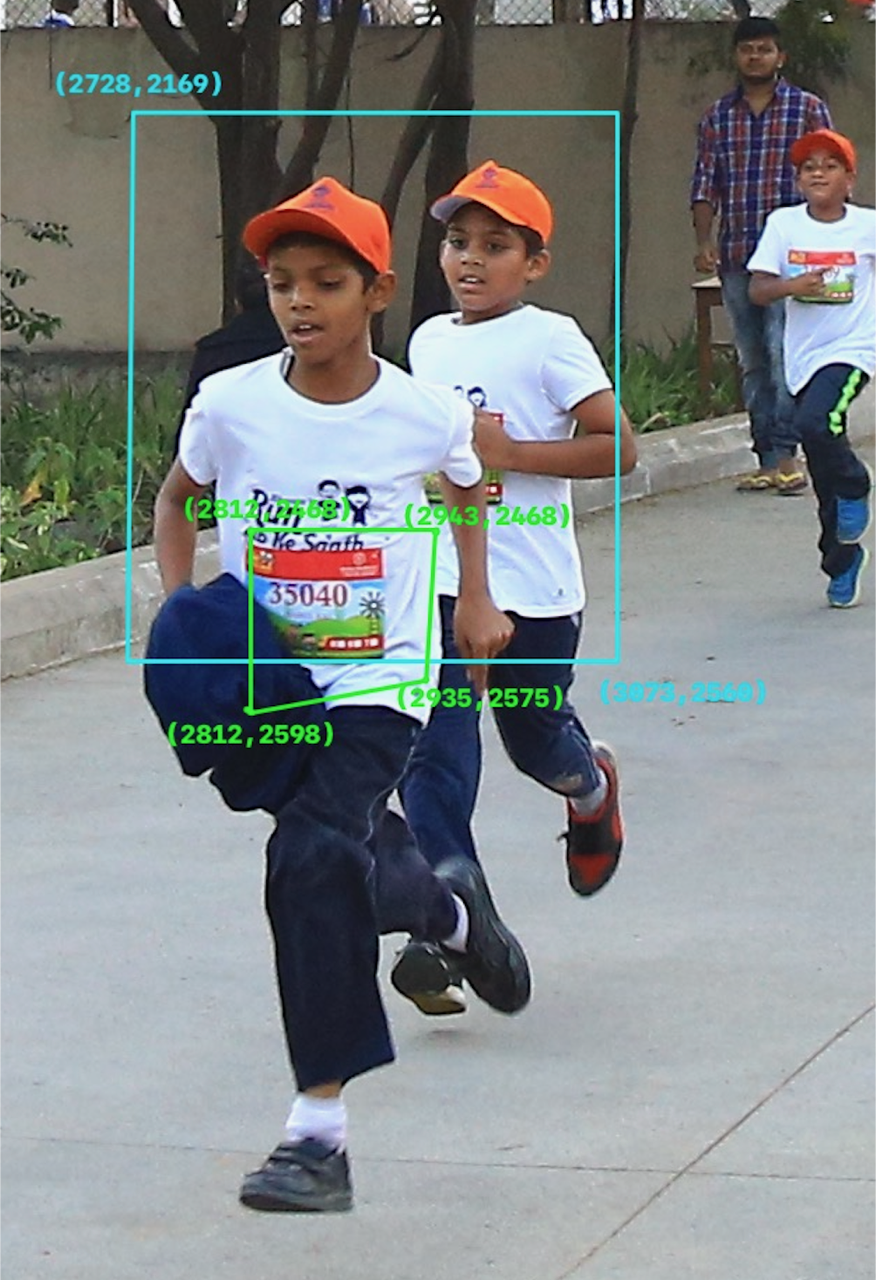
\includegraphics[width=\textwidth]{images/dataset/BadTagging_Overlap}
  \end{subfigure}
  \hspace{\fill}
  \begin{subfigure}[b]{0.3\textwidth}
    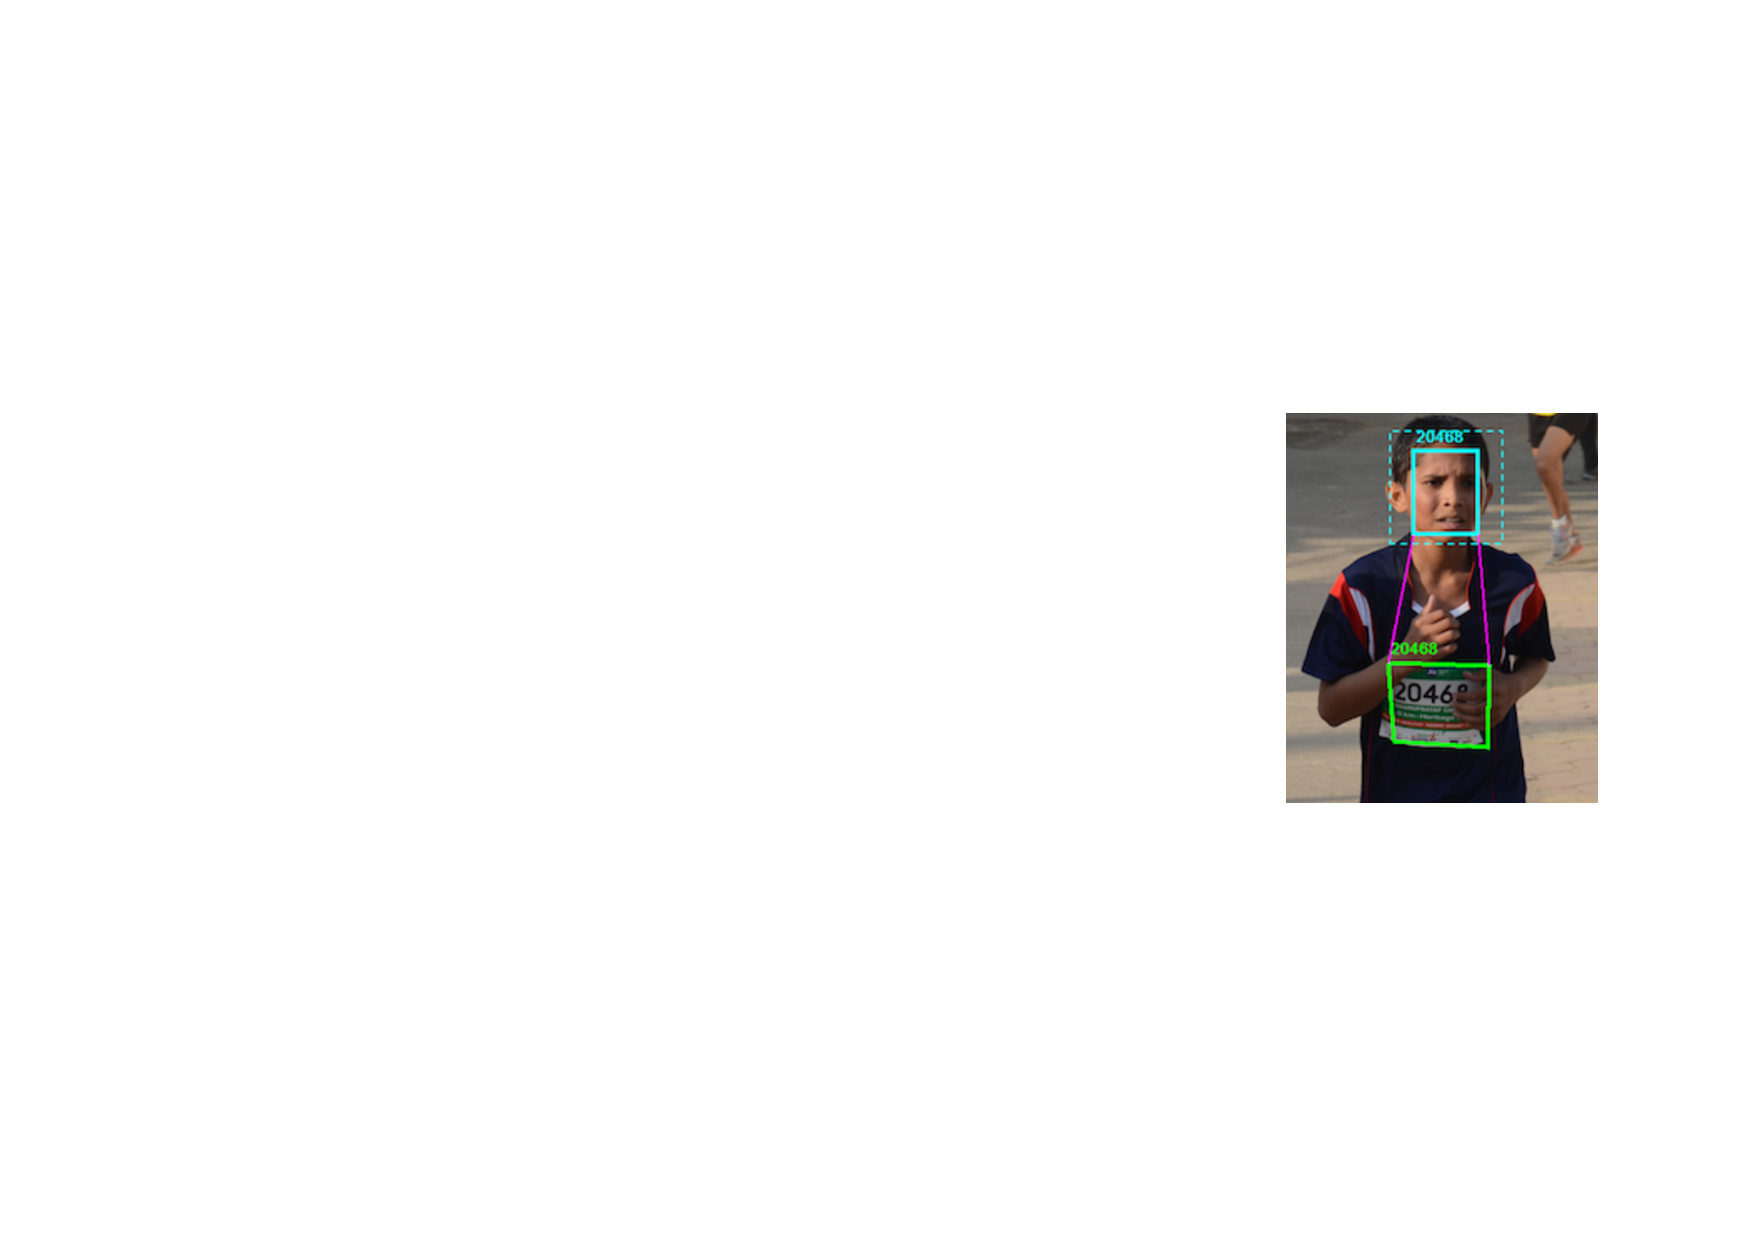
\includegraphics[width=\textwidth]{images/dataset/BadTagging_NotAroundFace}
  \end{subfigure}
  \hspace{\fill}  
  \begin{subfigure}[b]{0.2\textwidth}
    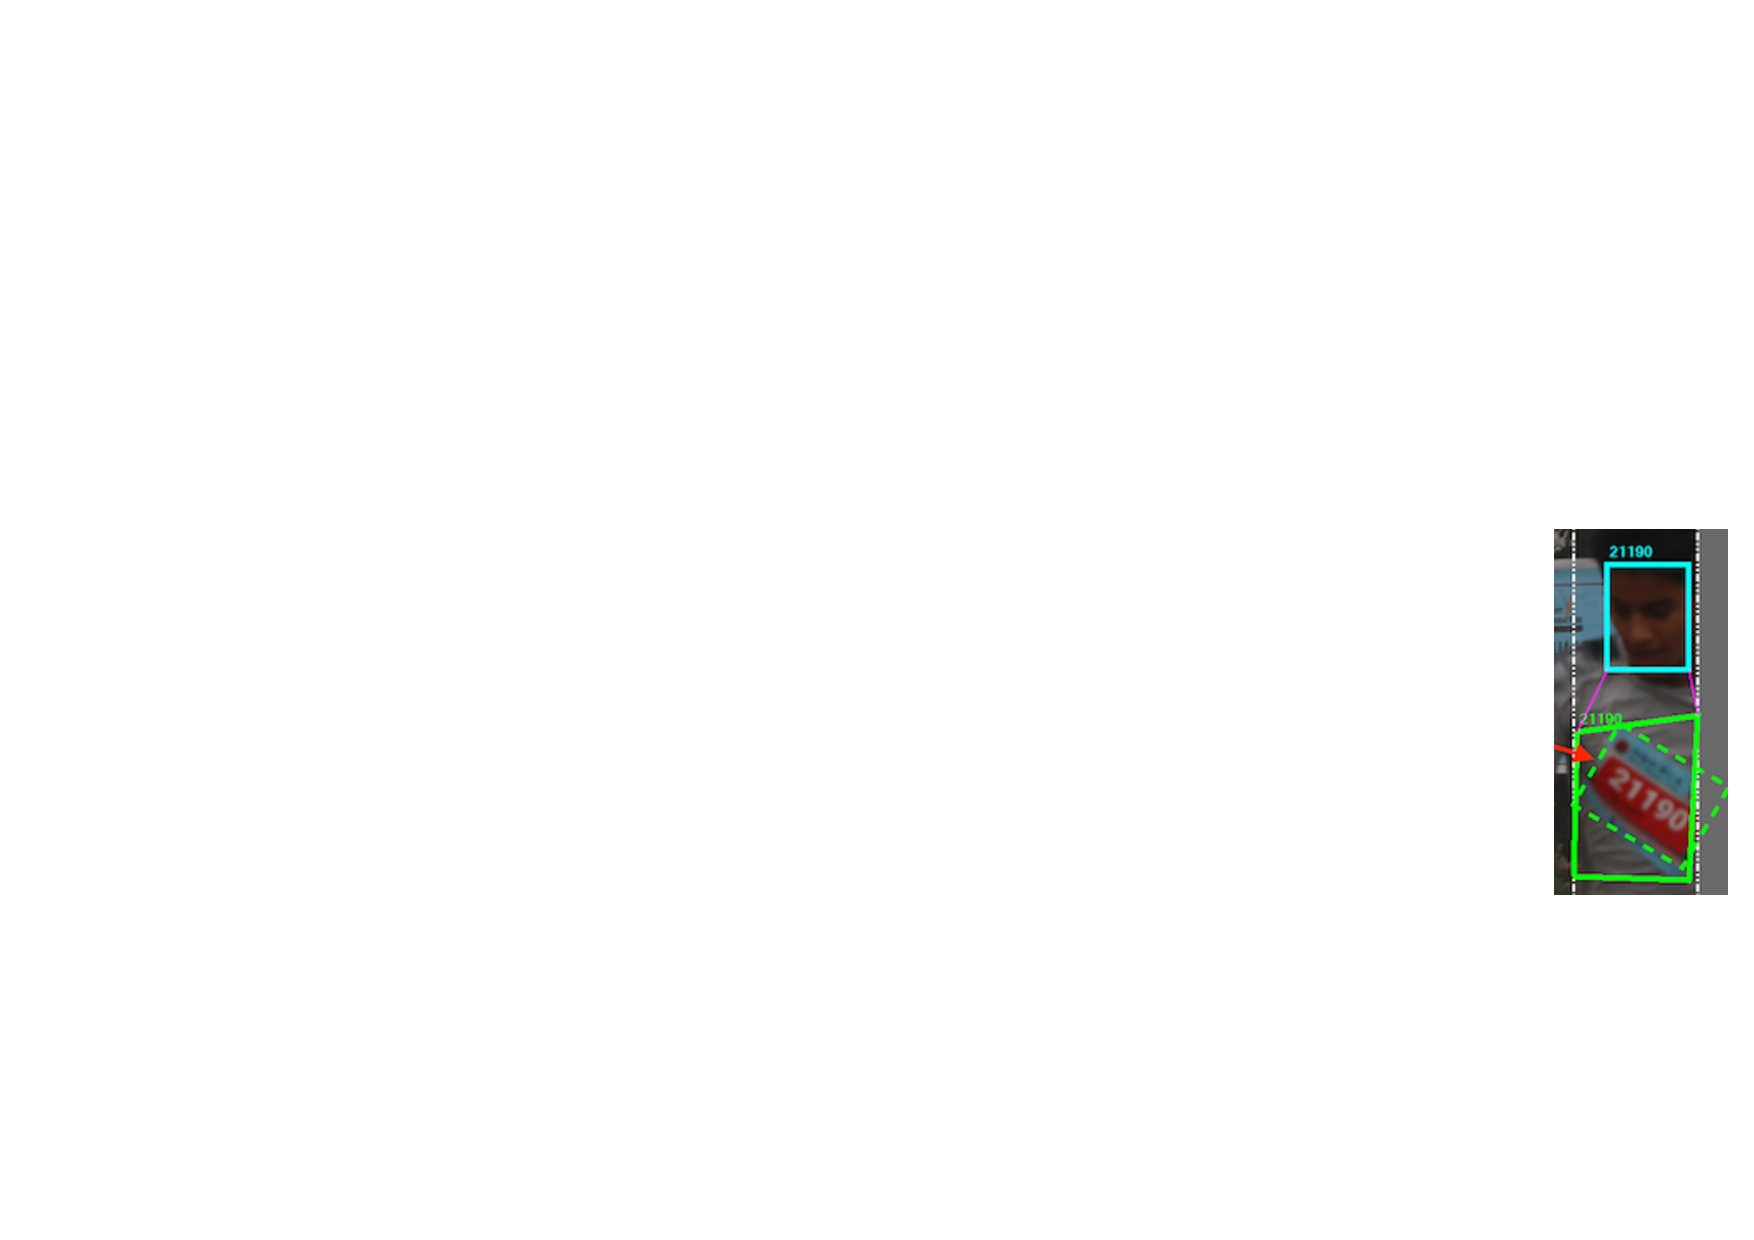
\includegraphics[width=\textwidth]{images/dataset/BadTagging_NotAroundBib}
  \end{subfigure}
  \hspace{\fill}
  
  \caption[Product testing issues identified]{Issues identified from rounds of external testing to the tagging team. Cyan lines indicate face regions, lime lines indicate bib regions, magenta lines indicate bib-to-face guidelines. \textit{Clockwise:} Face region is too far away from bib region; bib region is poorly marked (dotted lines expected); face region is too small (dotted lines expected); face region overlaps bib region.}
  \label{fig:dataset:issues_with_tagging}
\end{figure}

\subsection{Attributes}

Attributes exist as a means to capture further information about an annotation. We represent attributes in our metamodel as either derived or explicit. As stated in \cref{sec:dataset:architecture:what_to_capture}, those attributes which are required for the tagger to manually markup are explicit (i.e., manually must be added) whereas those that can be computed by the system are derived (i.e., inferred from explicit attributes). A useful example of derived attributes may be the bounding box and area that inferred from a polygon, both of which are key values required in training \glspl{nn}.
